% !TEX root = ../MasterThesis_goto_v1.tex

%%%%%%%%%%%%%%%%%%%%%%%%%%%%%%%%%%%%%%%%%%%%%%%%%%%%%%%%%%%%%%%%%%%%%%%%%%%%%%%%%%%%%%%%%%%%%%%%%%%%%
\chapter{深層学習を用いた崩壊点検出} \label{chap:VertexFinderwithDL}

本章では、本論文の主題である深層学習を用いた崩壊点検出について述べる。
前章の\ref{chap:Networks}. ネットワークでは崩壊点検出のためのネットワークとして、1. 飛跡対についてのネットワーク、2. 任意の数の飛跡についてのネットワークの二つのネットワークを導入した。
しかし、もちろんこの個々のネットワーク単体では崩壊点検出は実現できないため、これらを組み合わせたアルゴリズムが必要である。
そのようなアルゴリズムや前章までのネットワークについての総括を\ref{VFDL:AlgorithmofVFDL}節で行う。
また、このアルゴリズムではネットワークの出力に対する閾値などの幾つかのパラメータが存在するため、\ref{VFDL:TuneandPerformanceofVFDL}節では、それらパラメータの最適化について議論する。
同時に、どのような評価基準を用いて崩壊点検出の性能を判断するかについても、ここで述べる。
最後に\ref{VFDL:SummaryofVFDL}節では、以上によって実現された崩壊点検出について改めて性能の評価をまとめる。


%%%%%%%%%%%%%%%%%%%%%%%%%%%%%%%%%%%%%%%%%%%%%%%%%%%%%%%%%%%%%%%%%%%%%%%%%%%%%%%%%%%%%%%%%%%%%%%%%%%%%
\section{崩壊点検出アルゴリズム} \label{VFDL:AlgorithmofVFDL}

前章では個々のネットワークについて、比較や評価を行いネットワーク単体での性能について理解を深めた。
飛跡対についてのネットワークでは、SVの分離は非常に難しく、崩壊点のタネの段階での識別は現実的ではないということがわかった。
任意の数の飛跡についてのネットワークでは、個々の崩壊点に特化したネットワークが僅かながら性能が高いということを示した。
以上のことから、本研究では崩壊点のタネをPVとSVに分け、それぞれについて崩壊点の生成を行うこととした。
図\ref{3-3-2-2ImbalancedData}で示したように飛跡対についてのネットワークの出力はNCやPVが支配的であるため、SVが埋もれてしまうという課題がある。
このようなNCの組み合わせは、大半がPVとSVの組みから選ばれた飛跡対であると考えられる。
また、一般に事象中の飛跡においてPV由来の飛跡の割合が多いためPVから再構成する方が妥当である。
これらのことを踏まえ、図\ref{4-1-0-1VertexFinderAlgorithm}のような崩壊点検出アルゴリズムを提案する。

\begin{figure}[htbp]
 \centering
 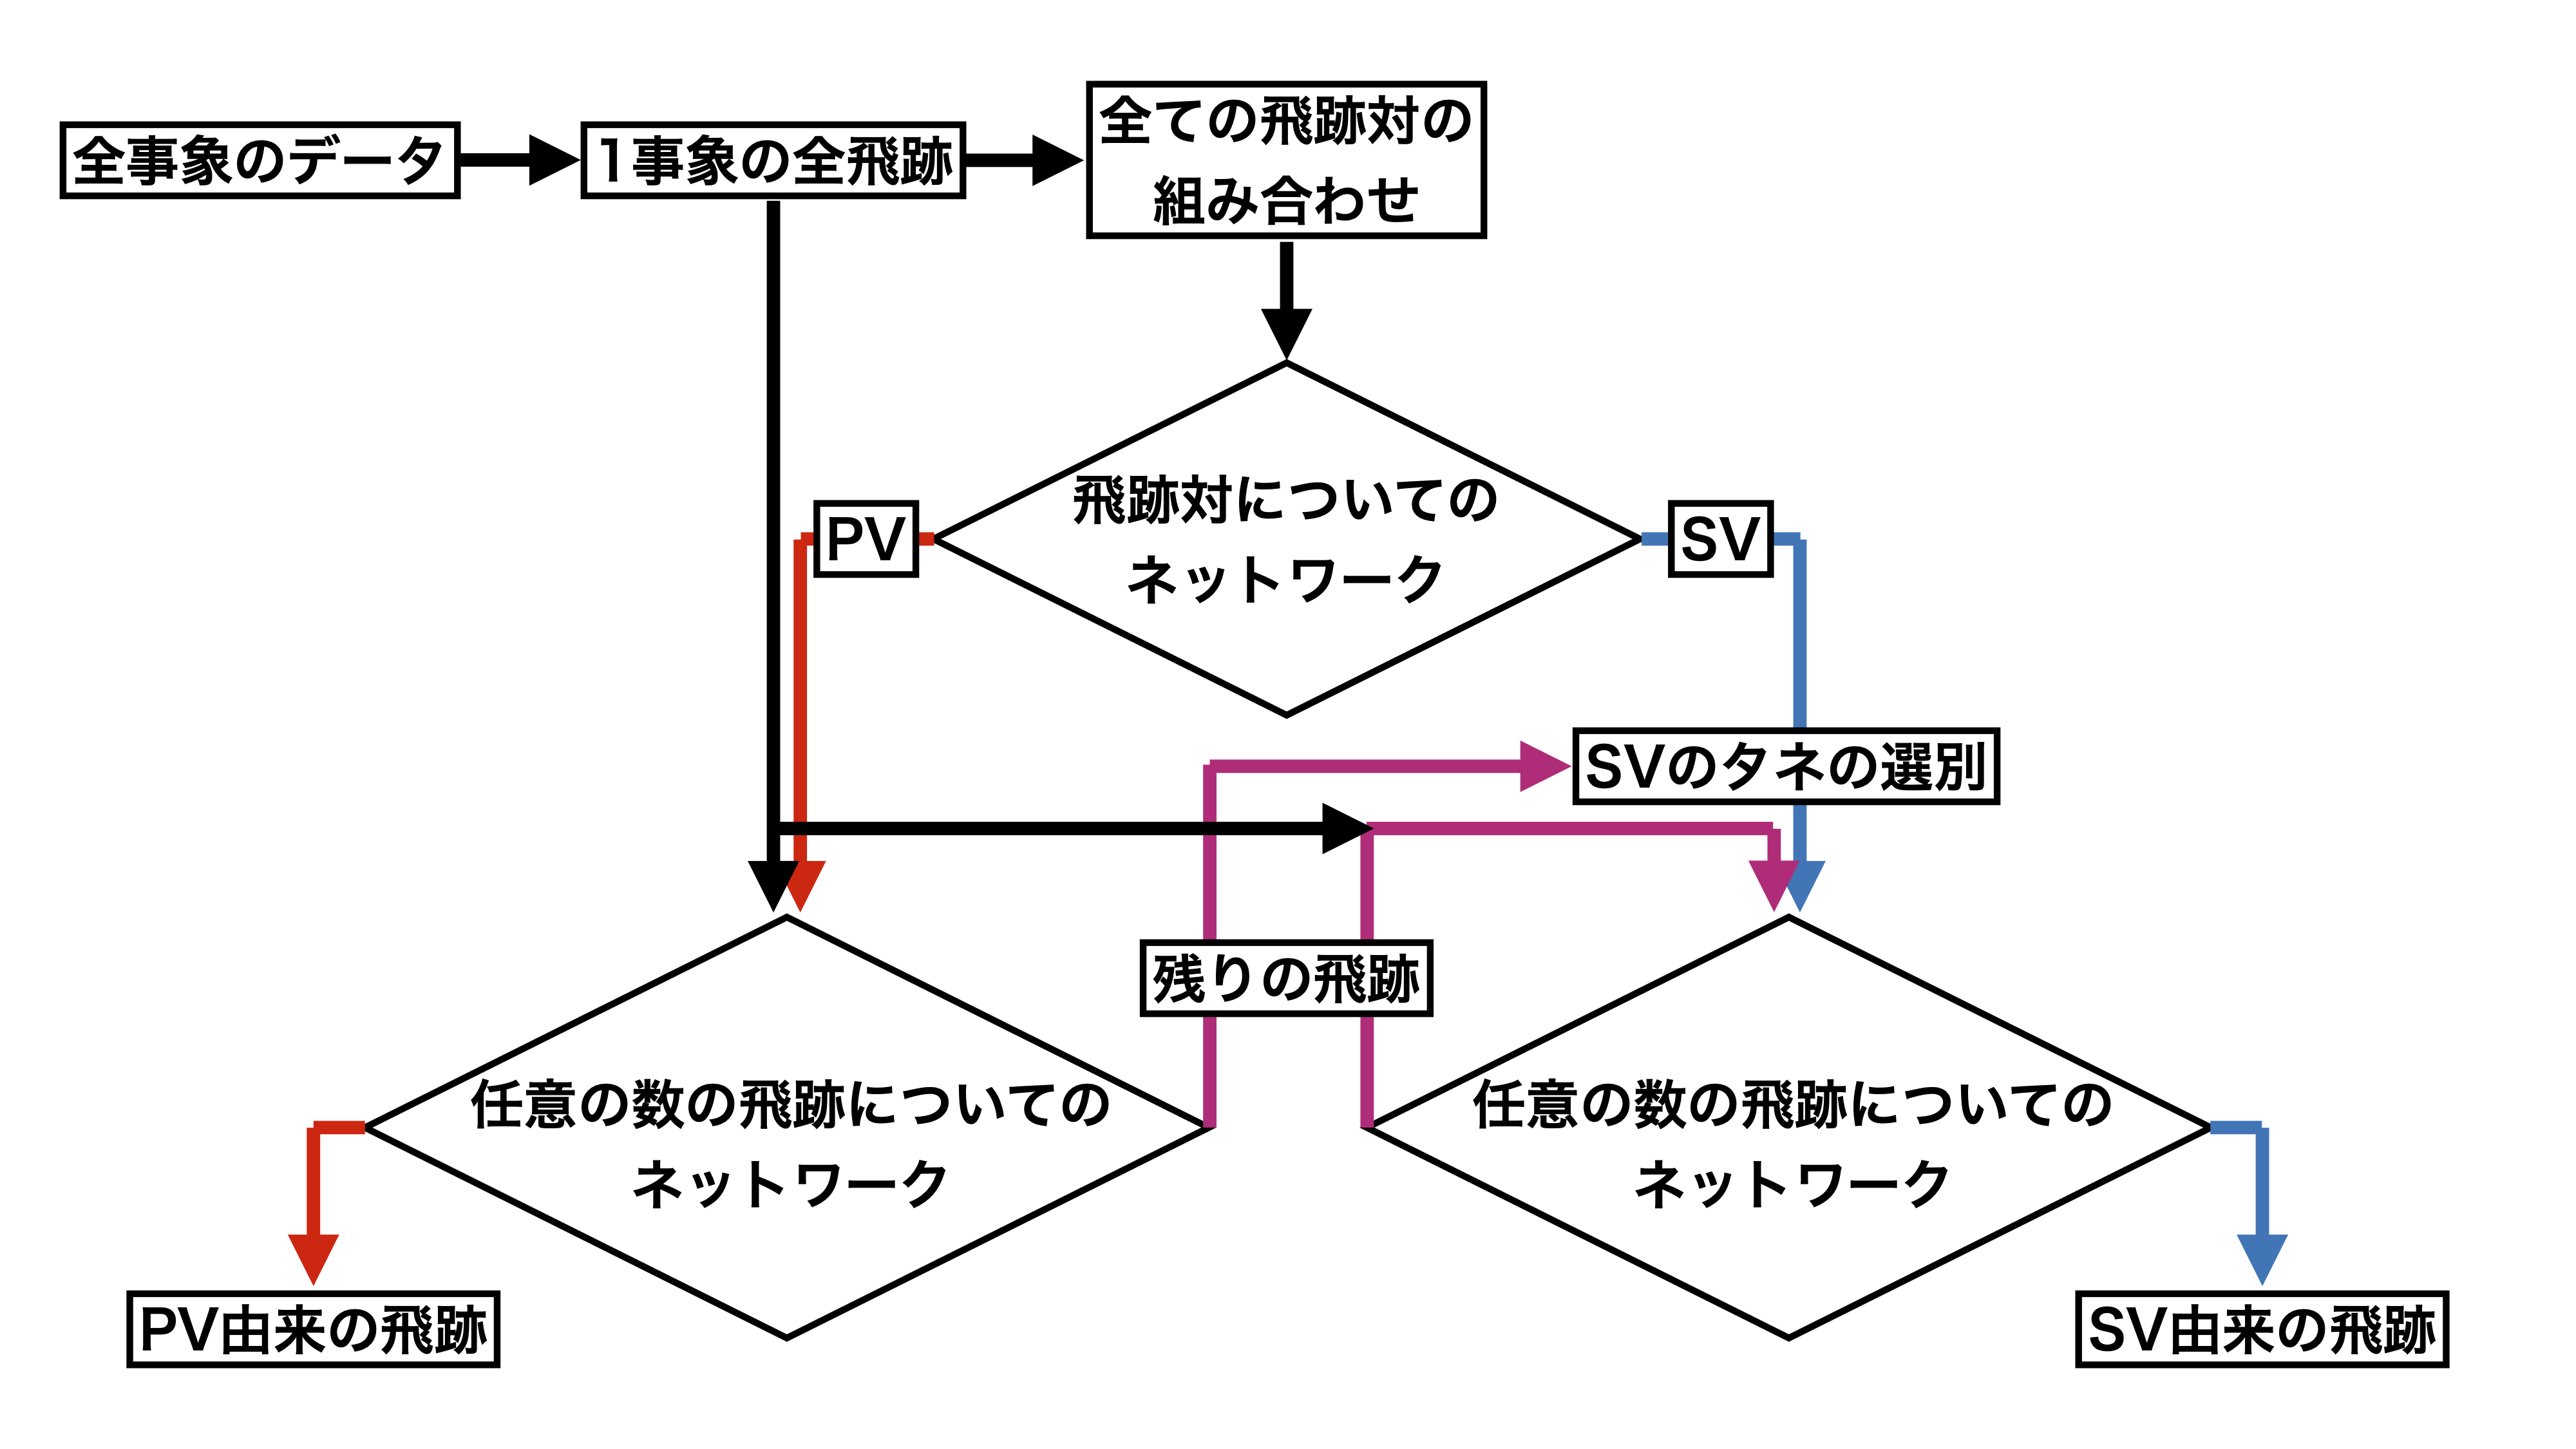
\includegraphics[width=0.9\textwidth, clip]{Figure/4VertexFinderwithDL/4-1-0-1VertexFinderAlgorithm.png}
 \caption{崩壊点検出アルゴリズム}
 \label{4-1-0-1VertexFinderAlgorithm}
\end{figure}

アルゴリズムは以下の手順で崩壊点の再構成を行う。

\begin{enumerate}
 \item 全事象から1事象分のデータを取り出し、全ての飛跡対の組み合わせを考える。
 \item それら飛跡対に対して、飛跡対についてのネットワークを使用し、崩壊点のタネの探索を行う。
 \item SVと判定された飛跡対について、選別を行いSVのタネを選ぶ。
 \item PVと判定されたタネについて、任意の数の飛跡についてのネットワークを用いPVの生成を行う。
 \item SVのタネとPV由来の飛跡の情報を用い、任意の数の飛跡についてのネットワークによってSVのタネが無くなるまでSVを生成する。
\end{enumerate}

手順1、2については飛跡対についてのネットワークの訓練データの作成や学習と全く同様の手順である。

手順3では、飛跡対についてのネットワークによって得られるSVCC・SVBB・TVCC・SVBCのスコアや崩壊点の位置を用いてより純度の高いSVのタネの集合を作成する。
したがって、SVCC・SVBB・TVCC・SVBCのスコアについての閾値や崩壊点の位置についての最適化が必要である。

手順4では、飛跡対についてのネットワークによって得られるPVのスコアに関して降順に並び替えたPVのタネに対して、個々に任意の数の飛跡についてのネットワークを用いPVを生成する。
ここでは、幾つのPVのタネを用いるかの最適化が必要である。
また一度以上、任意の数の飛跡についてのネットワークによって結合していると判定された飛跡をPV由来であると判断している。
この時の任意の数の飛跡についてのネットワークによって得られるスコアについての閾値についてもまた同様に最適化が必要なパラメータである。

手順5について、手順3で選別したSVのタネと手順4で得られたPV由来であると判定された飛跡の一覧を用いてSVの再構成を行う。
ここでは任意の数の飛跡についてのネットワークのデコーダー部に入力する飛跡から、再構成されたSV由来の飛跡を取り除いて行くことによって、再帰的にSVの生成が行われる。
SVのタネに含まれる飛跡はPV由来の飛跡の一覧になく、かつそれまでに生成したSV由来の飛跡の一覧にもないものを用いる。
このSVに関する任意の数の飛跡についてのネットワークのスコアも最適化が必要である。
また、再構成されたSV由来の飛跡の一覧にPV由来の飛跡が存在した場合は任意の数の飛跡についてのネットワークによって得られたスコアによって飛跡の争奪が行われる。
手順5はSVのタネが無くなるまで行われ、再構成されたSV由来の飛跡とPV由来の飛跡以外の飛跡は残りの飛跡とする。

以上が崩壊点検出のためのアルゴリズムである。
最適化が必要なパラメータを以下にまとめる。

\begin{itemize}
 \item 飛跡対についてのネットワークによって得られるSVCC・SVBB・TVCC・SVBCのスコアについての閾値
 \item 飛跡対についてのネットワークによって得られる崩壊点の位置についての閾値
 \item 使用するPVのタネの数
 \item PVの生成に関する任意の数の飛跡についてのネットワークによって得られるスコアについての閾値
 \item SVの生成に関する任意の数の飛跡についてのネットワークによって得られるスコアについての閾値
\end{itemize}

%%%%%%%%%%%%%%%%%%%%%%%%%%%%%%%%%%%%%%%%%%%%%%%%%%%%%%%%%%%%%%%%%%%%%%%%%%%%%%%%%%%%%%%%%%%%%%%%%%%%%
\section{崩壊点検出の最適化と評価} \label{VFDL:TuneandPerformanceofVFDL}

崩壊点検出の最適化では、まず、飛跡対についてのネットワークによって得られるSVCC・SVBB・TVCC・SVBCのスコアについての閾値と崩壊点の位置についての閾値の最適化を行う。
次に、使用するPVのタネの数、PV、SVの生成に関する任意の数の飛跡についてのネットワークによって得られるスコアについての閾値の最適化を行う。
前者はSVのタネの探索に関するパラメータ、後者は崩壊点の生成や全体性能についてのパラメータである。\\

1. SVのタネの探索\\

SVのタネを探索する上での評価基準は高い純度とある程度の効率である。
ここでは、SVのタネの効率や純度について、SVCC・SVBB・TVCC・SVBCのスコアの和に対する閾値と崩壊点の位置についての閾値を変化させ最適な値を探る。
ただし、崩壊点検出アルゴリズムではここから更にPV由来である飛跡を含むタネを除外する為、その純度は改善される考えられる。
そのような真のSVのタネの効率や純度は2. 崩壊点生成で確認する。
また、SVのタネの選別におけるPre-Selectionとして、飛跡対についてのネットワークでNC・PV・Othersと判定された飛跡対は取り除いている。
閾値とSVのタネの効率、純度の関係を図\ref{}に示す。
スコアについてはSVCC・SVBB・TVCC・SVBCの和を$0.5$から$1$まで$0.01$ずつ変化させ、崩壊点の位置については$10^{-2}$から$10^{2} {\mathrm mm}$まで対数スケールで$50$等分割した。

ここで効率や純度は次のように定義している。
したがって効率が$1$を超えてしまうことがある点に注意が必要である。


2. 崩壊点の生成\\

崩壊点の生成や全体性能についてのパラメータを最適化する為、崩壊点検出の性能の基準を定める必要がある。
そのような評価項目は飛跡での効率を用いている。
詳細な項目の基準を以下に示す。

\begin{itemize}
 \item MCPrimaryRecoSV : MC情報によってPV由来の飛跡であるとラベルされた飛跡の内、ネットワークがどの程度SVと判断してしまったか
 \item MCOthersRecoSV : MC情報によってOthersであるとラベルされた飛跡の内、ネットワークがどの程度SVと判断してしまったか
 \item MCBottomRecoSV : MC情報によってボトム・フレーバーのSV由来であるとラベルされた飛跡の内、ネットワークがどの程度SVと判断できたか
 \item MCCharmRecoSV : MC情報によってチャーム・フレーバーのSV由来であるとラベルされた飛跡の内、ネットワークがどの程度SVと判断できたか
\end{itemize}

更に、ボトム・フレーバー、チャーム・フレーバーのSV由来である飛跡については以下の評価を行う。

\begin{itemize}
 \item SameChain : 同一のチェイン由来の飛跡のみで構成されているか
 \item SameParticle : 同一の粒子由来の飛跡のみで構成されているか
\end{itemize}

ここでは、ボトム・フレーバー、チャーム・フレーバーのSVの内、同じボトム・ハドロンから生じたSVの組みをチェインと呼び、更に細かく個々のSVを粒子と呼んでいる (図\ref{4-2-0-1SameChainSameParticle})。
同一のチェイン、同一の粒子とはこれらのチェインや粒子を跨いで飛跡を選択しているかどうかを判断している。

\begin{figure}[htbp]
 \centering
 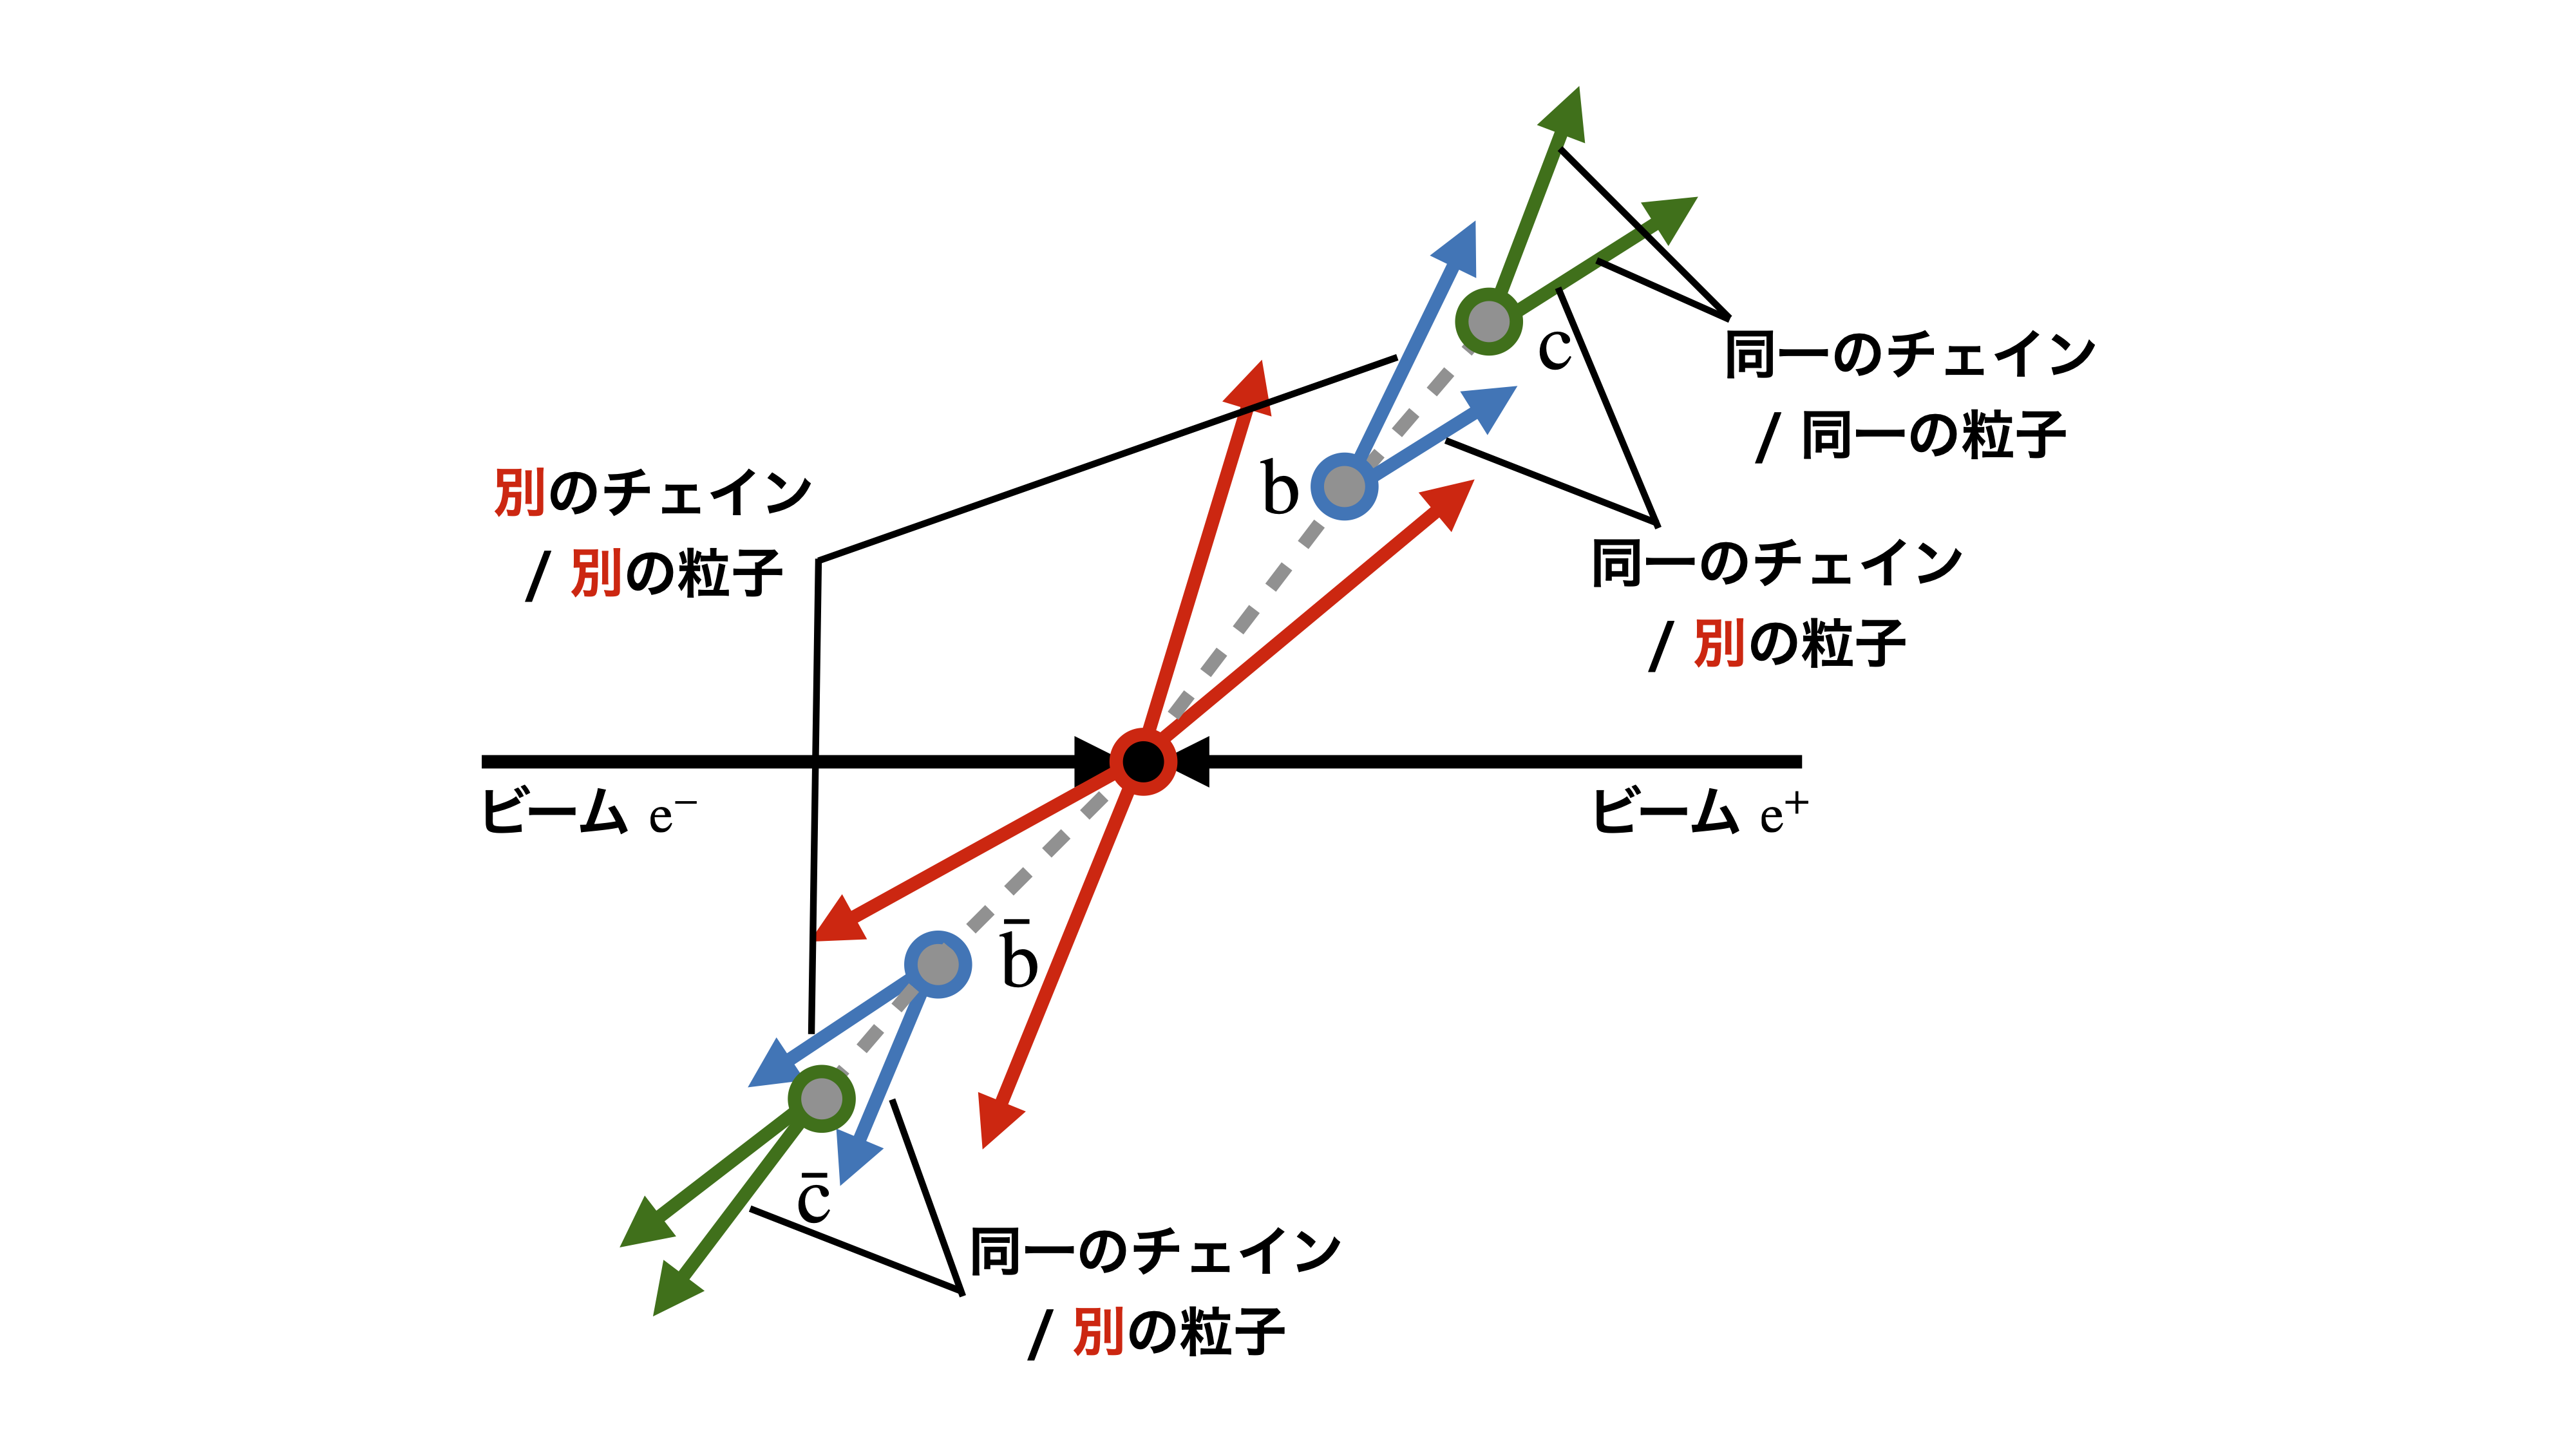
\includegraphics[width=0.9\textwidth, clip]{Figure/4VertexFinderwithDL/4-2-0-1SameChainSameParticle.png}
 \caption{同一のチェインと同一の粒子}
 \label{4-2-0-1SameChainSameParticle}
\end{figure}

これらの評価項目は前述した現行の手法であるLCFIPlusでの評価項目と同じものである。
また、同一のチェインなどの基準は終状態が終状態$\rm b\bar{b}$のものでしか起こり得ないことについても注意が必要である。
したがってこれらの評価は基本的には終状態$\rm b\bar{b}$のデータを用いて行うこととなる。

崩壊点の生成や全体性能についてのパラメータは使用するPVのタネの数、PV、SVの生成でのネットワークのスコアの閾値の三つである。
それぞれ三つのパラメータをPVのタネの数を$1$から$3$個まで、PV、SVのスコアの閾値を$0.5$から$0.95$まで変化させた時の各評価項目の値を図\ref{}に示す。
また、それぞれの評価項目の値は$100$事象についての平均を取っている。


%%%%%%%%%%%%%%%%%%%%%%%%%%%%%%%%%%%%%%%%%%%%%%%%%%%%%%%%%%%%%%%%%%%%%%%%


\section{崩壊点検出の性能} \label{VFDL:SummaryofVFDL}






















